% Created 2018-08-02 Thu 13:58
\documentclass[12pt, letterpaper]{paper}
\usepackage[utf8]{inputenc}
\usepackage[T1]{fontenc}
\usepackage{fixltx2e}
\usepackage{graphicx}
\usepackage{longtable}
\usepackage{float}
\usepackage{wrapfig}
\usepackage{rotating}
\usepackage[normalem]{ulem}
\usepackage{amsmath}
\usepackage{textcomp}
\usepackage{marvosym}
\usepackage{wasysym}
\usepackage{amssymb}
\usepackage{hyperref}
\tolerance=1000
\usepackage{tikz}
\usepackage{minted}
\usepackage{natbib}
\usepackage[margin=1in]{geometry}
\def\BigO{{\cal O}}
\renewcommand\maketitle{}
\DeclareMathOperator*{\argmin}{arg\,min}
\usepackage{caption}
\usepackage{subcaption}
\usepackage{mathtools}
\DeclarePairedDelimiter{\ceil}{\lceil}{\rceil}
\usepackage{bm}
\author{Timothy Schwieg}
\date{\today}
\title{A Structural Approach to Estimation of Valuations Randomly Distributed in Counter-Strike: Global Offensive}
\hypersetup{
  pdfkeywords={},
  pdfsubject={},
  pdfcreator={Emacs 25.3.1 (Org mode 8.2.10)}}
\begin{document}

\maketitle
\bibliographystyle{chicago}

\begin{titlepage}
\vspace{2.5cm}
\centering
{\scshape\LARGE University of Central Florida\par}
\vspace{1cm}
{\scshape Economics Department\par}
\vspace{2.5cm}
{\huge\bfseries A Structural Approach to Estimation of Valuations Randomly Distributed in Counter-Strike: Global Offensive \par}
\vspace{3cm}
{\Large\itshape Timothy Schwieg\par}
\vfill
Submitted for ECO 6936
\vfill

{\large \today\par}
\end{titlepage}


\section{Introduction}
\label{sec-1}
In the first-person shooter game \emph{Counter-Strike: Global Offensive},
players play online games against each other featuring various
versions of modern guns. Players can buy or earn skins for these
weapons, a recoloring of the weapon that is visible to both themselves
and anyone currently in the game. There are skins for virtually
every element of the game: guns, knives and gloves, with many being
very rare, and thus very expensive. These skins vary from re-coloring
to artistic designs. They are purely cosmetic and have no influence on
the outcome of the game.

As an incentive for playing, players can randomly receive an item as a
reward at the end of a match. These items can come in two possible
forms: common skins and weapon cases. The weapon cases are lotteries
that contain various weapons with fixed and known probabilities. If one
believes that each individual has fixed preferences between each of the
items contained in the boxes, a utility function over lotteries and
there exists unobserved heterogeneity between individuals in their
risk preferences, then this induces a distribution of valuations for the
lotteries. A large number of potential items contained in
each of the boxes exist, as there are many varieties to a single item.

These items are issued randomly over time to players, and the process
with which they are distributed is of interest. When a new case is
introduced to the market, one would like to see if there is a
change in the probability of receiving the older cases, as well as if
there are adjustments made over time by Valve, the company running the
game. Since these items are distributed randomly, there is no reason to
believe that they are in any way efficiently allocated. In order to
allow for an efficient outcome, these items are traded at
market. This market allows those with the highest valuation to end up
with the item, reaching an efficient allocation. The market is
available to all players with a steam account and is public. 

I seek to impose a strong structure on how these items are distributed
to players, and determine the nature of the valuations as well as how
many players are active in the market and how many enter or leave the
market over time. These primitives can then be extracted to determine
future policy decisions made about the implementation of newer items
into the game. 

\section{Model}
\label{sec-2}

For any given item, assume that there is a mass of consumers who have
valuations based on some distribution $F_V$. With some exogenous
probability, some consumers are endowed with an item with probability
$\bm{\xi}$. Consequently, the same distribution of valuations in those
endowed as well as those who are not endowed, even if there are
different numbers of people who are endowed. 

Because the process of granting items is random, it is in no way
efficient. The individuals who value the good most do not necessarily
receive it under the current function. In order to achieve this
efficiency, a market is implemented, taking the form of a double
auction.

It is known that double auctions  converge rapidly to a competitive
environment; see \cite{Efficiency}. The data pulled are relatively poor for extracting
valuations from the bids, as for much of the data the bids are not
observed; as a result attempting to identify valuations from the bids
would not work well. Even though the result is certainly possible for
double auctions under conditions such as sealed-bid, and one buyer and
seller, there has been no identification, based on a dominant or
equilibrium argument in the continuous double auction. See: \citet*{DoubleAuc} 

Consequently, I shall abstract from the dynamics and the
mechanism of the double auction, and due to the large amount of
traffic, focus on its convergence into a competitive market. If the
market is efficient, then a matching between buyers and
sellers obtains after the trades where those with the highest
valuations have the items. Since there is large amount of buyers in
each time period, we will use he rapid convergence to assume a
competitive equilibrium without much ado.

\subsection{Matching Problem}
\label{sec-2-1}
I examine the competitive market in the context of a matching
problem, Following the model by Shapley and Shubik of perfectly transferable
utility. \citet*{LitReview}  Since it is known that the planner's problem of maximizing total
welfare, and the decentralized market are equivalent for this problem,
one can examine either interchangeably to provide motivation for the
problem. 

The surplus generated by any exchange between a buyer and a seller is
given by the valuation of the buyer minus the valuation of the
seller. A central planner, who wishes to maximize the total surplus
then faces the question of finding a (partial) matching between buyers
and sellers such that the surplus generated is maximized. For some
arbitrary $I$ buyers and $J$ sellers:

\begin{align*}
\max_{\alpha_{i,j}} & \sum_{i=1}^I \sum_{j=1}^J \left ( V_i - V_j \right ) \alpha_{i,j }\\
\text{subject to: } & \forall j, 1 \leq j \le J \quad \sum_{i=1}^I \alpha_{i,j} \leq 1 \\
& \forall i, 1 \leq i \leq I \quad \sum_{j=1}^J \alpha_{i,j} \le 1 \\
\end{align*}

The constraints serve to require that each individual make at most one
exchange. One desirable result is that this linear program is always
maximized at integer values of $\alpha$. This ensures that the solution
contains no partial matching.  Of interest as well is the dual of
the problem, specified below.

\begin{align*}
\min_{x,j} & \sum_{i=1}^I x_i + \sum_{j=1}^J y_j \\
\text{subject to: } & \forall i,j; \quad 1 \leq j \leq J, \quad 1 \le i \leq I\\
& x_i + y_j \geq V_i - V_j 
\end{align*}

The solution to this problem form the shadow prices of the exchange,
or the amount of surplus that a buyer or seller takes based on their
type. These allow for the price to be computed directly.

\subsubsection{Results}
\label{sec-2-1-1}
One important thing to note about the objective function is that it is
the buyer's valuation less the seller's valuation. At the time of the
matching, $V_i$, $V_j$ are known and fixed, and not random. The
objective function is both super-modular and sub-modular. For this
matching problem, this implies that both positive assortative mating
and negative assortative mating are supported. \cite{LitReview} After
some inspection, one can see that even though the process will
determine which of the sellers and buyers match, any permutation of
the matches is just as optimal. This means that any maximizer of the
primal is not unique.

That said, the dual of the problem does have a unique solution, as it is
the shadow price for the type of the seller and the buyer. These
values are the producer and consumer surplus for each type. Since it is
a competitive equilibrium, there is one price supported, as the good
is homogeneous, and the matching is occurring between valuations for the
good. The seller's valuation plus his shadow price will be equal to
the competitive price for all sellers who do exchange. 

For equal-sized buyer and seller valuations, this gives the intuitive
result that the lower half of the distribution of sellers will sell to
the upper half of the distribution of buyers, and we will have the
efficient result. As the size of the seller's mass shrinks, with the
rarity of the item increasing, a higher proportion of the sellers
choose to sell, and the receiving end of the distribution of buyers
shrinks, as the price increases. This is demonstrated below for
valuations that are distributed normally, with mean 35, and standard
deviation of 10. One tenth of the population is endowed with the item.
The equilibrium price is calculated by taking the seller's valuation
plus his shadow price.

If one considers the decentralized market version of the problem, all
buyers are indifferent between the sellers they choose, as they must
give up the producer surplus to the seller, and as a result face a
constant price to buy from any seller type. 

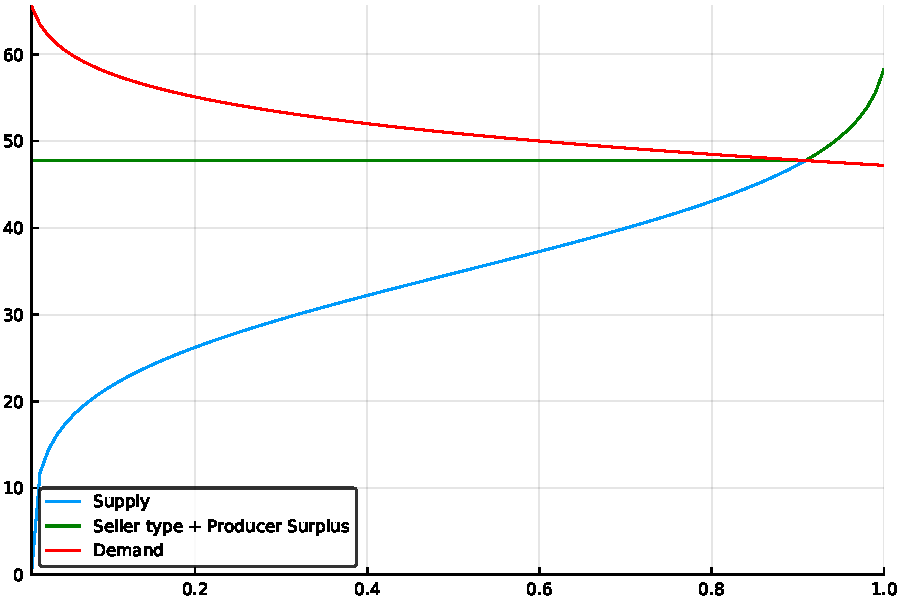
\includegraphics[width=.9\linewidth]{../Scripts/oneTenth.pdf}

The distribution of buyers has become truncated by the difference in
the number of buyers and sellers. To maintain the efficient outcome,
only the top $10$ percent of the buyers are able to purchase, and $90$
percent of the sellers are now selling.

Within the context of this matching model, the change in the relative
sizes of the population of suppliers acts to truncate the buyers
rather than lower the supply. It is important to note that these are
not exactly supply and demand in the normal sense, as instead of
quantity, the $x$-axis is the proportion of the sellers that exchange.

\subsubsection{Equilibrium}
\label{sec-2-1-2}
As a result of the lens in which this market is viewed, a slightly
different sort of equilibrium obtains. Although all the desirable
properties of an equilibrium hold, notably efficiency, and being in
the core, we are only examining exchanges in one good, so it remains a
partial equilibrium. \cite{LitReview}

Assume that the valuations of the players are distributed normally, as
in the examples above. Then the supply function can be written as $q^s
= N \xi\Phi \left ( \frac{ p - \mu }{\sigma} \right )$ and the demand function
can be written as: $q^d = N \left ( 1 - \xi\right ) \left [ 1 - \Phi \left
( \frac{ p - \mu }{ \sigma } \right ) \right ]$, $\xi$ is the percent of people
endowed with the item. In equilibrium, the quantity of buyers and
sellers are equal:

\begin{align*}
\xi \Phi \left ( \frac{ p^* - \mu }{\sigma} \right ) &= (1-\xi) \left [ 1 - \Phi \left
( \frac{ p^* - \mu }{\sigma} \right ) \right ]\\
p^* &= \mu + \sigma \Phi^{-1} ( 1- \xi)\\
\end{align*}

The price supported by the market is the average
valuation plus a component that depends on the rarity of the
item. Essentially, the price is controlled by some
universal notion of value, such as the design of the skin, as well as
a rarity element that drives price up or down depending on how easy it
is to obtain.

\subsection{Dynamics}
\label{sec-2-2}
The data are ordered according to time intervals, so the process must
be estimated dynamically. Consider a series of time intervals, in
which there is the matching device described above. In each interval, a percentage of
the population is awarded the item, and the matching device functions
to distribute efficiently.

Firstly, consider the model with no entrants. After the initial
exchange, those that do not have the item are random attributed the
item again, but their distribution is no longer the initial
distribution, it has been conditioned on losing the top portion of its
mass. Therefore the distribution of those that are possible sellers is
a mixture of this truncated distribution, and the top portion that
left the potential buyers. In this model, the top portion of
those that have the item will never sell it, as the valuations of
those that do not are all strictly below them: consider the
seller distribution to be a percentage of the buyers. The process then
repeats, albeit with a slightly truncated portion of the valuation
function. 

This model also more captures more elements of the market than the
original, as it can explain the behavior observed of a high initial
price, slowly dropping to some equilibrium level. With an explanation
of the dynamics of the process in place, we can look at the entire
lifetime of the item, and only have to control for the truncation of
the valuations for the demand. As long as there is no entrance of
individuals into the model, the price will necessarily decrease.


\subsubsection{Specification}
\label{sec-2-2-1}

For each time period $t$, the drop rate to individuals estimated is
given by: $\xi$$_{\text{t}}$. The price observed in that period is $p_t$. In the first
time period, everything proceeds according to the previous
model. In the second time period however, allow the top $\xi$$_{\text{0}}$ percent to
exit the model. There are $N(1-\xi_0)$ people remaining, of which $\xi$$_{\text{1}}$ have
received the item, so the mass of suppliers is: $\xi_1 (1-\xi_0)N$. The mass
of the buyers is: $(1-\xi_1)(1-\xi_0)N$. It should be noted that the
distribution of both the supply and demand is binomial, with its mass,
and probability of purchase at each price.

\begin{align*}
\Pr \left [ V_2 < v | V_1 < F_V^{-1}( 1 - \xi_0 )^{} \right ] &=
\frac { F_V ( v ) }{  F_V ( F_V^{-1} ( 1 - \xi_0 ) ) } = \frac{ F_V (v)
}{1 - \xi_0}\\
\mathbb{E} \left [ q_2^s \right ] &= N ( 1-\xi_0 )\xi_1 \left [ \frac{\Phi \left ( \frac{ \log ( p_t ) - \mu }{\sigma} \right )}{ 1 - \xi_0 } \right ]\\
\mathbb{E} \left [ q_2^d \right ] &= N ( 1-\xi_0 )(1-\xi_1) \left [ 1 - \frac{ \Phi \left ( \frac{
\log ( p_T ) - \mu }{ \sigma } \right ) }{ 1 - \xi_0 } \right ]
\end{align*}

One may continue the process, noting that with each truncation, there
is a multiplication of $(1-\xi_t)$ in the denominator of the valuation
function.

\begin{align*}
\mathbb{E} \left [ q_T^s \right ] &= N \prod_{t=1}^{T-1} (1-\xi_t ) \xi_T \frac{\Phi \left ( \frac{ \log ( p_T ) - \mu }{\sigma} \right )}{ \prod_{t=1}^{T-1} ( 1 - \xi_t ) }\\
\mathbb{E} \left [ q_T^d \right ] &= N \prod_{t=1}^{T} ( 1- \xi_t ) \left [ 1 - \frac{ \Phi \left ( \frac{
\log ( p_T ) - \mu }{ \sigma } \right ) }{ \prod_{t=1}^{T-1} (1 - \xi_t ) } \right ]\\
\log \left ( p_T^* \right ) &= \mu + \sigma \Phi^{-1} \left [ \prod_{t=1}^T ( 1 - \xi_t ) \right ]\\
q_T^* &= N \xi_T \prod_{t=1}^T ( 1 - \xi_t )\\
\end{align*}



\subsection{Market Entry}
\label{sec-2-3}

Although the percentage endowment model does describe several of the price
processes quite well, it struggles to rationalize the nearly constant
quantity of items sold in each period. One way to explain that is to
allow for market entry over time.

Consider the case in which the number of entrants in the market is not
held constant, and instead new entrants to the market have a different
distribution from older ones. The distribution of the buyers in the
following period is now a mixture distribution. Since one can now
find a buyer of the highest valuation, it is possible that sellers who
had previously bought might be willing to sell again. Consequently, the
entire seller's distribution must be considered as well, as a mixture
of the highest valuations, and the individuals that have just become
endowed.

After the first exchange of items, $\lambda$$_{\text{0}}$
percent of $N$ people enter the market, drawing their valuations from a
potentially different distribution $E_t$. Then the endowment process is
repeated, and exchange occurs. After this process, $\lambda$$_{\text{1}}$ percent of the
$N(1+\lambda_0)$ people enter the market. That is, $\lambda_t$ is the proportion of the
inhabitants of the market that enter the market in time period
$t$. However, they enter the market after the exchange has
occurred. This ensures that there is no entrance in the first time
period where it would be indistinguishable from $N$.

The distribution of buyers and sellers remains binomial. Since all
sellers are possible sellers now, the distribution and mass of the
buyers and sellers has become noticeably more complex. The mass of the
sellers is now the sum of the mass of the buyers times the percent of
people endowed in each time interval. That is, in time period one, the
sellers received $N \xi_0$ mass, and the mass of the buyers was:
$N(1-\xi_0)$. However, then $N\lambda_0$ people arrived, and for time period one
the buyers had mass: $N( 1 -\xi_0 + \lambda_0)(1-\xi_1)$, and the sellers had mass:
$N \xi_0 + N(1-\xi_0 + \lambda_0)\xi_1$.

The mass of the buyers and the sellers continues on this trend and is
given by:

\begin{align*}
M_B(T) &= ( 1 - \xi_T ) \left [ M_B(T-1) + \lambda_{T-1} \prod_{t=1}^{T-2}( 1 + \lambda_t )N \right ] \\
M_S(T) &= N \prod_{t=1}^{T-1} ( 1 + \lambda_t ) - M_B (T)\\
\end{align*}

In each time period, it is assumed that the market clears and,
therefore, the price observed in each time period determines the
percent of people that choose to purchase. All buyers with valuations
above the price choose to purchase, and all sellers with valuations
below the price choose to sell. Since there is entry into the
market, the distribution will no longer simply be truncated. The
truncated distribution of people who chose not to buy will be mixed
with an untruncated distribution of individuals who enter the
market. The incoming distribution may be significant enough to
drive the price up; thus it is possible that those who bought the item in a
previous time period may wish to sell it as the price is driven
upward. Thus, one must consider everyone who has received the
item in the supply, rather than just the individuals who received it
in the current time period.

If the price increases from time $T$ to time $T+1$, we know therefore that
all purchasers must be entrants to the market, as everyone who could
have bought it in the previous time period would have. If the price
decreases from time $T$ to time $T+1$, then the sellers distribution must
only contain people who received it during this time period. These two
facts imply that our supply and demand functions will be kinked, and
analytic representations of price and quantity will be impossible to
obtain except for trivial cases.

It is assumed that at each time period, the market is in equilibrium, so
the previous valuation function evaluated at the previous equilibrium
price signals the percent of the buyer's mass that purchased the
item. Let $E_T (p)$ be the distribution function for the valuations of
a person entering the market at time $T$. Let $B_0 = S_0$ be the initial
valuation functions.

\begin{align*}
B_T (p) &= \frac{ B_{T-1 }(p_{T-1}) }{ B_{T-1 }(p_{T-1}) + \lambda_T } \min \left \{ 1, \frac{ B_{T-1} ( p ) }{B_{T-1 }(p_{T-1 })} \right \}
 + \frac{ \lambda_1 }{ B_{T-1 }(p_{T-1}) + \lambda_T } E_T (p) \\
S_T (p) &= \frac{ M_S(T-1) }{ M_S(T) } \max \left \{ 0, \frac{ B_{T-1}(p) - B_{T-1}( p_{T-1} ) }{ 1 - B_{T-1} ( p_{T-1} ) } \right \} + \frac{ M_S(T) - M_S(T-1)_{} }{M_S(T)} B_T (p)\\
\end{align*} 

$B_T(p)$ and $S_T(p)$ are strictly increasing functions of p, so the
intersection between $B_T(p), S_T (p)$ is uniquely defined. In the case when
$\lambda_t = 0$ this is the dynamic model covered previously. The moment
conditions we shall invoke are implied by the competitive equilibrium:
Namely, expected values be equal and equal to quantity sold.

\begin{align*}
M_B(T) B_T(p_T^*) &= M_S (T) S_T (p_T^*)\\
M_B(T) B_T (p_T^*) & = q_T^*\\
\end{align*}



\section{Source of Data}
\label{sec-3}
The data has been mined from the Steam Community Market API, which
provides a purchase history for every item on the market, down to the
hour for the last thirty days and daily for the rest of the lifetime
of the item. It does not provide a record of every purchase, just the
quantity sold in that time period as well as the median price they
were sold at. The price data is only accurate to the cent, and
features a price floor of \$0.03. The selling mechanism is a K-double
auction where the seller always receives his bid. Buy and sell orders are
placed, and then matched based on price and time spent waiting in queue.


The data is price and quantity sold data of items on the Steam
Community Market for the game \emph{Counter Strike: Global
Offensive}. Players in game earn items random that they can sell on
the market or open themselves. Most rare items are earned via opening
of dropped \emph{loot boxes} that are then opened by players via purchasing
of a key. These boxes can be earned by playing or received randomly
from players who are watching professional games. The probabilities of
the drops are not known or even estimated well, as they change
depending on many factors including time. They are one primitive that
we seek to estimate. 

Once a box has been obtained, the probability of receiving an
item is well documented as required by Chinese Law. Each item has a
certain grade of rarity, for example the AK-47 Redline has a rarity
level of Classified which means that there is a 3.2 percent chance of
receiving a Classified item in the crate. All items of equal quality
contained in the crate have the same probability of being dropped by
the crate.

Many variants of each item exist. Each item has a quality
ascribed to it, the float of the item. This describes the wear on the
item, and is distributed uniformly on the interval 0-1. On the market
the items are split into intervals: Battle-scared, well-worn,
field-tested, minimal wear and factory new. Each quality is a separate
listing on the market with a separate price. In addition to each item
having a quality type there is also a ten percent chance of each item being
labeled as StatTrak, which also distinguishes the value of a
weapon. This means that each item has ten possible different variations
all with different probabilities of being obtained. Some rare items,
usually knives and gloves may have more or less quality variants, but the
amount and probabilities are known, and can easily be determined by
checking if there is a market history for the item.

The probabilities for each condition are as follows:
\begin{center}
\begin{tabular}{ll}
Float & Condition\\
0.00 - 0.07 & Factory New\\
0.07 - 0.15 & Minimal Wear\\
0.15 - 0.38 & Field-Tested\\
0.38 - 0.45 & Well-Worn\\
0.45 - 1.00 & Battle-Scarred\\
\end{tabular}
\end{center}
Each item has a 10 percent chance of being StatTrak if that item has StatTrak
enabled. float values are distributed uniformly, making the
probability calculations simple.

The rarity of a skin also controls its probability of being
dropped in a particular lottery. These rarities are set by Valve, and
are specified for each crate. They rank from gold (very rare) to blue
(common). The probabilities of getting an item of a rarity is given as follows:
\begin{center}
\begin{tabular}{rl}
Probability & Rarity\\
0.0026 & Special (Gold)\\
0.0064 & Covert (Red)\\
0.032 & Classified (Pink)\\
0.1598 & Restricted (Purple)\\
0.7992 & Mil-spec (Blue)\\
\end{tabular}
\end{center}
In each box there are several items of each rarity, each one is
equally likely to be found when the lottery is realized.

Each box contains some subset of these items that is known, and the
market value of each item at a particular time period is also known,
so the expected value, or any other modified version of a valuation of
the lottery can easily be calculated.

\section{Estimation}
\label{sec-4}
Initially, consider estimates of the model without entry. In each time
period, the distribution of supply and demand is binomial. These
distributions are independent, and the difference between two binomial
distributions that are not independent is difficult to estimate using
likelihood methods. Consequently, the generalized method of moments
will be utilized. Since the price is uniquely defined in each time
period, as is the quantity supplied, the question of estimation is
feasible.

For period $T$, there exists two moment conditions specified,
one for price, and one for quantity. Under the specification for the
model:

\begin{align*}
F_V \left ( p_T^* \right ) &= \prod_{t=1}^T ( 1 - \xi_t )\\
q_T^* &= \xi_T \prod_{t=1}^T ( 1 - \xi_t )\\
\end{align*}

This provides us with $2T$ moment restrictions on the model, and allows
for estimation of up to $2T$ parameters.

A distinction must be made between observations and time
periods. The data are divided into the median price and quantity
sold in each day, and the question of how many data points are in a
time period must be answered. For the purposes of the estimation in this paper,
I shall use five observations per time period. If there are $N$
observations, then there are $T = \ceil*{ \frac{ N }{5} }$ time
periods. This arises from the need for no serial correlation between
the data points in order to exploit the statistical properties of the method.

For the model specified with $T$ time periods, and for a distribution of
prices of log-normal, there are two parameters for the distribution, and
$T$ parameters for $\bm{\xi}$. There are $2T$ moment restrictions, so the model
is in fact over-identified. This allows us to test the specification
for our model using the Sargan-Hansen J-test.

\subsection{Complications}
\label{sec-4-1}

One important complication is that there exists a price-floor in the
market. No item is able to be sold at less than \$0.03, this means
that for all data points where the price is at this floor, the
equilibrium condition is not binding. All that one can say is that the
equilibrium price must be below the price floor. This censored
condition may be written as $p^* < p_T$. This is equivalent to: $\max\{
p^* - p_T, 0 \} = 0$. The equilibrium quantity is also not represented
by the data when the price is censored. The only condition that is
binding is that the quantity demanded at the price is the given
quantity when the price floor is binding. One can rewrite the two
conditions using the primitives of the model to give the binding
price-floor moment conditions:

\begin{align*}
\max \left \{ \prod_{t=1}^T ( 1 - \xi_t ) - \Phi \left ( \frac{ p_T^* - \mu }{\sigma} \right ), 0 \right \} &= 0\\
N \prod_{t=1}^T ( 1 - \xi_t ) \left [ 1 - \frac{ F_V ( p_T^* ) }{ \prod_{t=1}^{T-1} ( 1 - \xi_t ) } \right ] - q_T^d &= 0\\
\end{align*}

The maximum function is not differentiable at zero, where the
optimal value of our function is located. To overcome this, a
differentiable alternative to the maximum function will be used: 
\begin{equation*}
\max \{ x,y \} \approx \frac{ 1 }{\rho} \log \left [ \exp ( \rho x ) + \exp ( \rho y
) \right ] \quad \text{ for some } \rho > 0
\end{equation*}

One important aspect of the data that the theory does not represent
well is the path of the equilibrium quantity. Under the currently
defined model, the equilibrium quantity is a necessarily decreasing
function. Quality paths in the data follow a nearly constant
path. One way to handle this is to seek a different setting where the
equilibrium quantity can be viewed as a percent of the starting number
of people in the market. This can be rationalized by imagining that
after each transaction, the sellers re-enter the market with the
truncated valuation distribution. This means that there is always $N$
people available at each iteration of the market, but the distribution
continues to be truncated as before. This leaves the price moment unaffected.

\begin{equation*}
q_T^* = N \xi_T ( 1 - \xi_T )
\end{equation*}

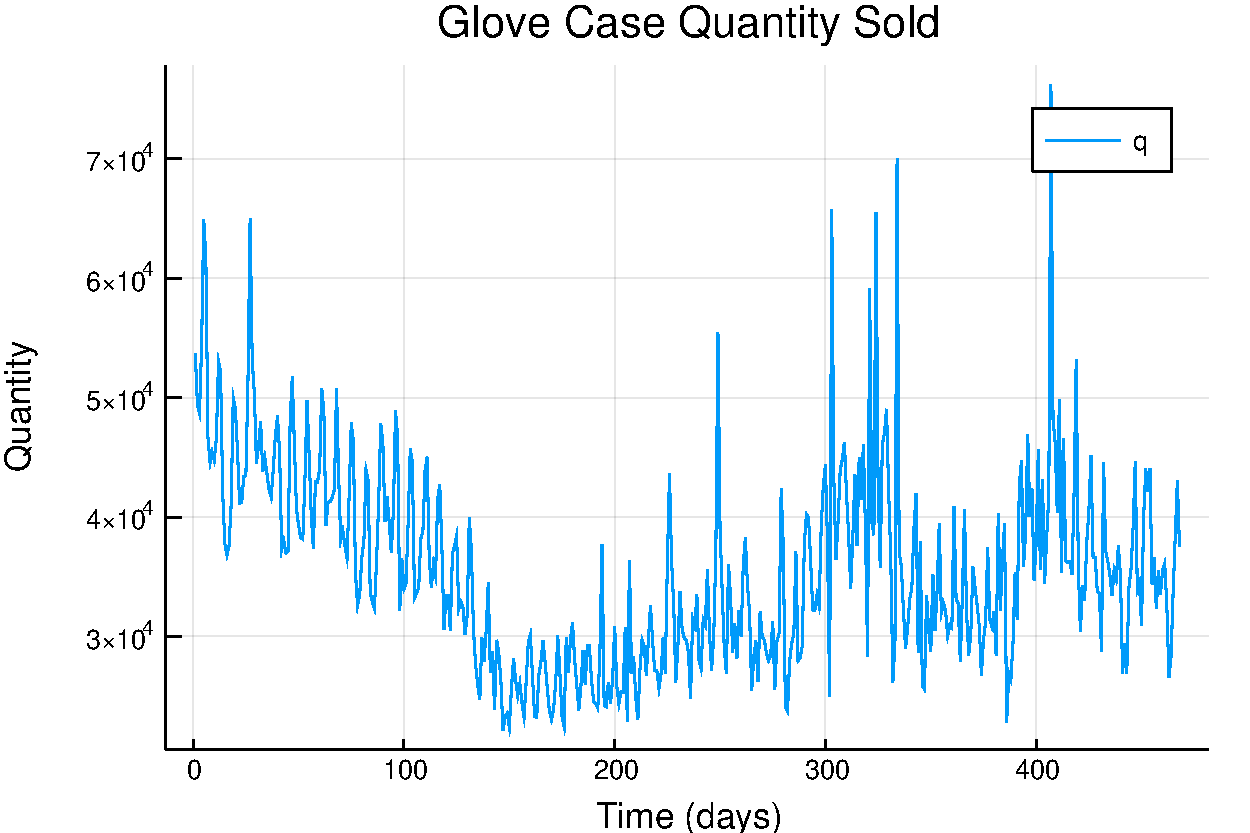
\includegraphics[width=.9\linewidth]{../Figures/Cases/Cases2/GloveCase_Quant.pdf}

This specification permits  estimation of quantities sold that all
remain on the same order of magnitude, as opposed to the strictly
decreasing quantity path specified in the original specification.


\subsection{Implementation}
\label{sec-4-2}
Consider a function $g(Y_t ,\mu,\sigma,\bm{\xi})$ which gives the moment condition for
each time period, evaluated at the $t^{th}$ element in that time
period. Under the Null Hypothesis that this model fits the data, then
the expected value of this function is zero.

\begin{equation*}
\mathbb{E}[ g( Y_t, \mu, \sigma, \bm{\xi}) ] = 0
\end{equation*}

I sought to estimate the parameters $\mu$, $\sigma$, $\bm{\xi}$ by minimizing the sample
analog of this with respect to a quadratic form of weighting matrix
W. The sample analog is formed by averaging the data found contained
in each time period.  $\bm{\hat{m}} ( \mu, \sigma, \bm{\xi}) = \frac{ 1 }{ M } \sum_{m=1}^M g(
Y_m, \mu, \sigma, \bm{\xi} )$. Combine the parameters of the model into a vector
$\bm{\theta}$. The goal then becomes to estimate a value of $\hat{\bm{\theta}}$ by
minimizing the quadratic form of $\bm{\hat{m}}( \bm{\hat{ \theta}} )$ with respect to
matrix $\bm{W}$.

\begin{equation*}
\bm{\hat{\theta}} = \argmin_{\bm{\theta}} \quad \bm{\hat{m}}( \bm{\theta} )' \bm{W} \bm{\hat{m}}( \bm{\theta} )
\end{equation*}

The choice of $\bm{W}$ is selected by first choosing a positive definite
matrix $\bm{W}$, and estimating the model, and then estimating the matrix by
the following method:

\begin{align*}
\bm{\hat{\theta}_i} &= \argmin_{\bm{\theta}} \quad \bm{\hat{m}}( \bm{\theta} )' \bm{\widehat{W}_{i-1}} \bm{\hat{m}}( \bm{\theta} ) \\
\bm{\widehat{W_i}} &= \left [ \frac{1}{M} \sum_{m=1}^M g(Y_m, \hat{\bm{\theta}}_{i-1} ) g( Y_m,\hat{\bm{\theta}}_{i-1}  )' \right ]^{-1} \\
\end{align*}

This process is then continued until the value of $\theta_{i-1}$ is a
minimizer for $\bm{\widehat{W_i}}$. This iterated GMM estimator is invariant to the
scale of the data, which is important in this model, as the price and
the quantity data are of wildly different magnitudes \cite{hall2005generalized}. This method is also asymptotically equivalent to the
Continuous Updating Efficient GMM, but does not have as many numerical
instabilities.

This process is complicated by $\bm{\widehat{W_i}}$ being of rank
$M$. If the matrix is not of full rank, then it is not invertible, and
one cannot estimate the model. In order to ensure that it has full
rank, the process is regularized by adding a positive number times the
identity matrix to ensure that $\bm{\widehat{W_i}}$ is both positive definite
and invertible. However, the asymptotic properties of the J-test
require that the matrix $\bm{\widehat{W_i}}$ be converging in probability to the
true variance matrix. As a result, we divide our positive number added
by the number of observations in each time period, allowing for our
change to converge to 0 in probability.


The model was estimated using the code found in the file
\texttt{dataTest2.jl} using the programming language Julia. Utilizing the
package \texttt{Optim.jl}, the objective function was minimized using the
BFGS algorithm. This ensured that numerical problems that could arise
out of calculations of inverting a small hessian were avoided. Several
of the fits are shown below. Gradient calculations were made using
Forward Automatic Differentiation, see: \citet*{ForwardDiff}.

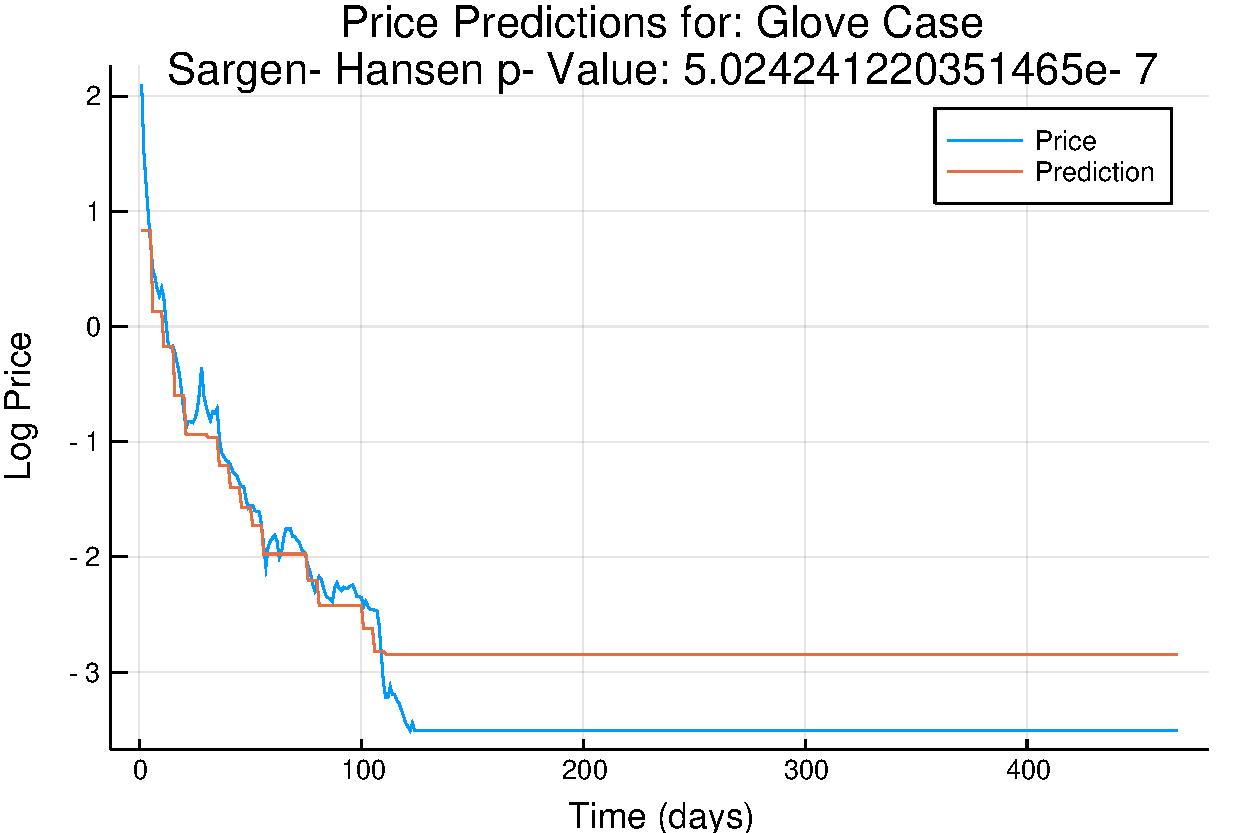
\includegraphics[width=12cm]{../Figures/Cases/Cases3/GloveCase.pdf}

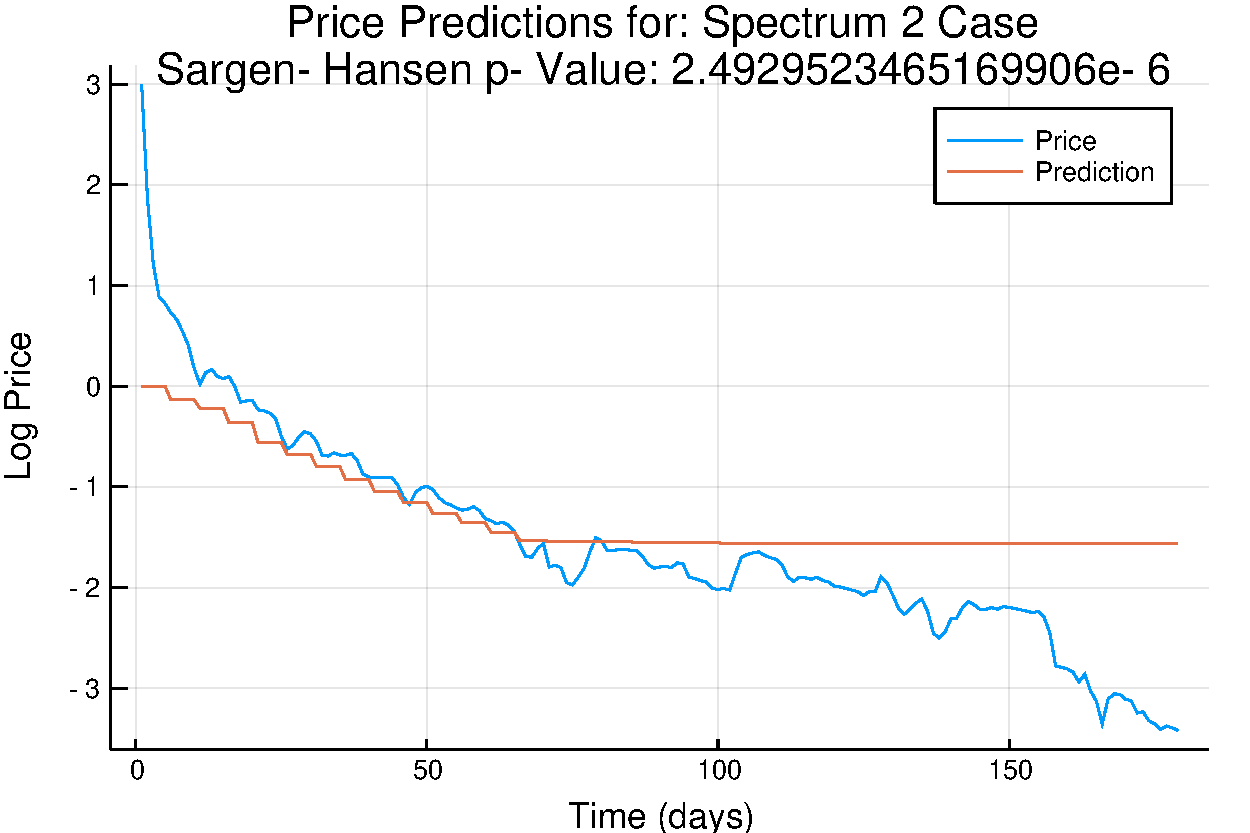
\includegraphics[width=12cm]{../Figures/Cases/Cases3/Spectrum2Case.pdf}

One important note on the price predictions is that the model is able
to predict the price path relatively well at the start, but begins to
struggle with matching the price in the latter half of the model. This
is due in part to the specification which gives undue control over the
price path to the earliest values of $\bm{\xi}$, causing the early
under-estimation of the price in the Spectrum 2 Case. Dominating the
latter part of the model is numerical problems. Even using the
exponential of sums of logarithms, the value of $\prod_{t=1}^T ( 1- \xi_t )$
still becomes ill-behaved numerically.

When there is lots of variability, leading itself to upward trends in
the price, the model can struggle trying to be able to incorporate the
data into its structure.

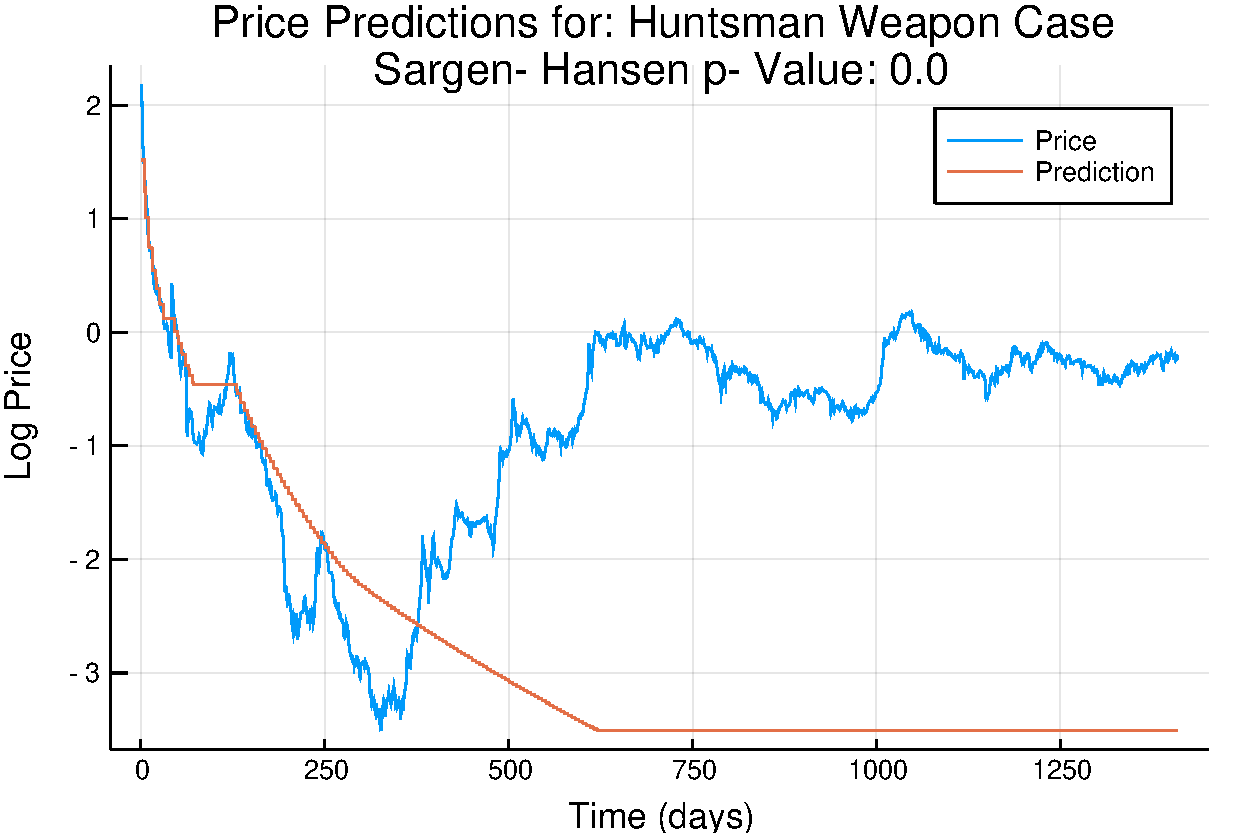
\includegraphics[width=12cm]{../Figures/Cases/Cases3/HuntsmanWeaponCase.pdf}

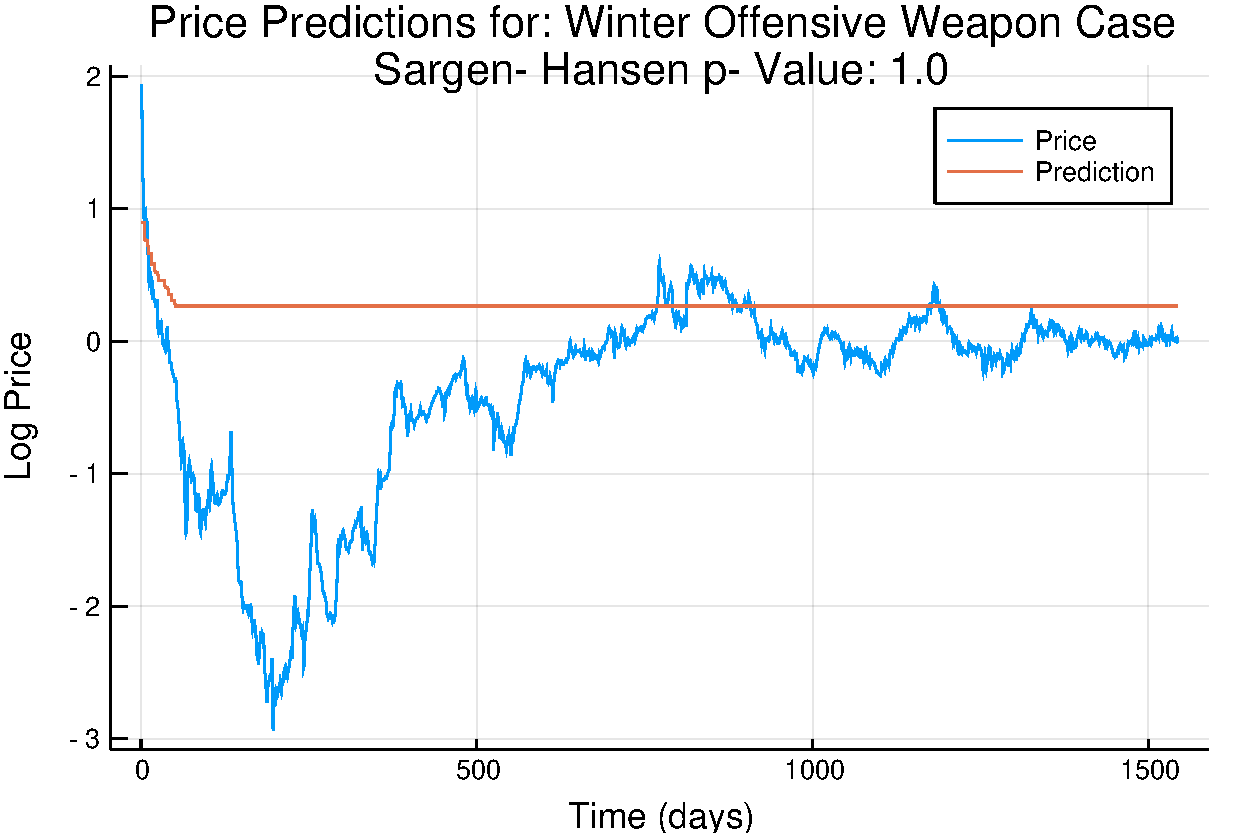
\includegraphics[width=12cm]{../Figures/Cases/Cases3/WinterOffensiveWeaponCase.pdf}

Even though the model struggles greatly with large increases in price, and
has no way of incorporating them into the primitives, sharp decreases
in the price are also difficult for the model to handle. In this
model, large decreases in the price require a large number of
individuals endowed with the item in that time period, something which
must also be supported by the quantity data.

\subsubsection{Numerical Complications}
\label{sec-4-2-1}
Two problems exist with the model as currently estimated: The sensitivity to
the initial value as well as the magnitude of the zero condition on
the moments.

The core issue with estimation in this dynamic system is that each
time period involves parameters from all the previous time
periods. This gives the estimated values of the endowment in the first
time periods enormous effect on the fit of the model. This also means
that the relationship between the different values of $\bm{\xi}$ is highly
complex and nonlinear. As a result of the nonlinearity, there are many
saddle points contained in the geometry.

To complicate matters is the form of $\widehat{\bm{W}}$. Since there are so few
data points in each time period, $\widehat{\bm{W}}$ relies on the
regularization to be positive definite and invertible, the optimization problem is
not well formed. One alternative would be to follow a simulation
sampling process to arrive at the minimum value. The process followed
in this paper is to test based on several different initial values of
$\mu$ and $\sigma$, and the minimum of those will be treated as the global
minimum. This does not guarantee that the process will converge to the
global minimum.  This creates problem using the iterative method of
forming $\widehat{\bm{W}}$, as optimization mishaps in the first instance are
compounded into an improperly formed covariance matrix that does not
need to even be positive definite.

These problems stem from the magnitude differences between the two
types of moment conditions. The price moment condition, which means on
the order of magnitude between negative three and three, and the quantity moment which
is on the magnitude of $30000$. While the final iteration of $\widehat{\bm{W}}$ is
invariant to differences in magnitudes of the moments, problems formed
in the initial optimization problem can manifest themselves, preventing
the routine from reaching the global minimum.

Since it is known that the limit of $\widehat{\bm{W_i}}$ is invariant
to differences in magnitudes between the components of $g_t$,
that means that one can adjust the magnitudes of the moments to allow
for the optimization routine to converge to the true minimum in the
early instances. As a result, the quantity moment is divided by $N$ in
order to place it on a magnitude with the price moment. This allows
for the price moments to impact the optimization routine in the first
few instances.

As a result, the moments used in estimating the procedure in each time
period are as given:

\begin{alignat*}{2}
 \quad & \exp \left [ \sum_{t=1}^T \log ( 1 - \xi_t ) \right ] - &\Phi \left [ \frac{ \log ( p_T^* ) - \mu }{ \sigma }  \right ] &= 0 \\        
 \quad & \exp \left [ \sum_{t=1}^T \log ( 1 - \xi_t ) \right ] - &\frac{q_T^*}{N} 
    &= 0
\end{alignat*}

For numerical stability, $\prod_{t=1}^T ( 1 - \xi_t )$ has been replaced by $\exp
\left [ \sum_{t=1}^T \log ( 1 - \xi_t ) \right ]$, which is much more stable when
dealing with small and large values of $\bm{\xi}$. On a numerical note, since
full identification requires that $\xi \in (0,\frac{1}{2})$. $\bm{\xi}$ will be
parametrized using a logistic function. In order to maintain that $\sigma$
will always be strictly positive, it will be parametrized according to
an exponential function, and $\mu$ will be parametrized by a logistic
function simply to reduce saddle points caused by large $\mu$ and $\sigma$. $N$
will not be parametrized throughout the model.

Using these specifications, estimation of the model remains a question of
unconstrained optimization, and though it is poorly specified and
difficult to minimize globally, the problem is, in principle,
solvable. Only one serious numerical concern remains.

The order of price constraint is not very representative of the
magnitude of the error in the predictions in price. Currently, the
moment requires a sufficiently small difference between the cdf of the
valuations of the buyers that have ramined in the market and the
product of the endowments. This creates problems when relatively large
differences in prices create relatively small differences in this
moment. This can lead to solutions where the price does not tend to
zero in the limit. This is caused by the model fitting the quantity
moment well but the relatively large difference in the price moment
having a small effect on the price moment condition. Sadly, applying
the inverse cdf transform to the function eliminates many of the ideal
properties required for optimization. The inverse cdf is not defined
analytically, and while its derivative is given by the composition of
the reciprocal of the derivative and the inverse function, this
formulation performed extremely poorly numerically, preventing
converge of any kind. The problem remains, causing there to be higher
than reasonable prices when the model is attempting to fit the
quantity evenly. This can cause problems such as in the Spectrum Case,
pictured below, where a large difference in the price is taken as a
small difference between the cdf and $\prod_{t=1}^T ( 1 - \bm{\xi} )$

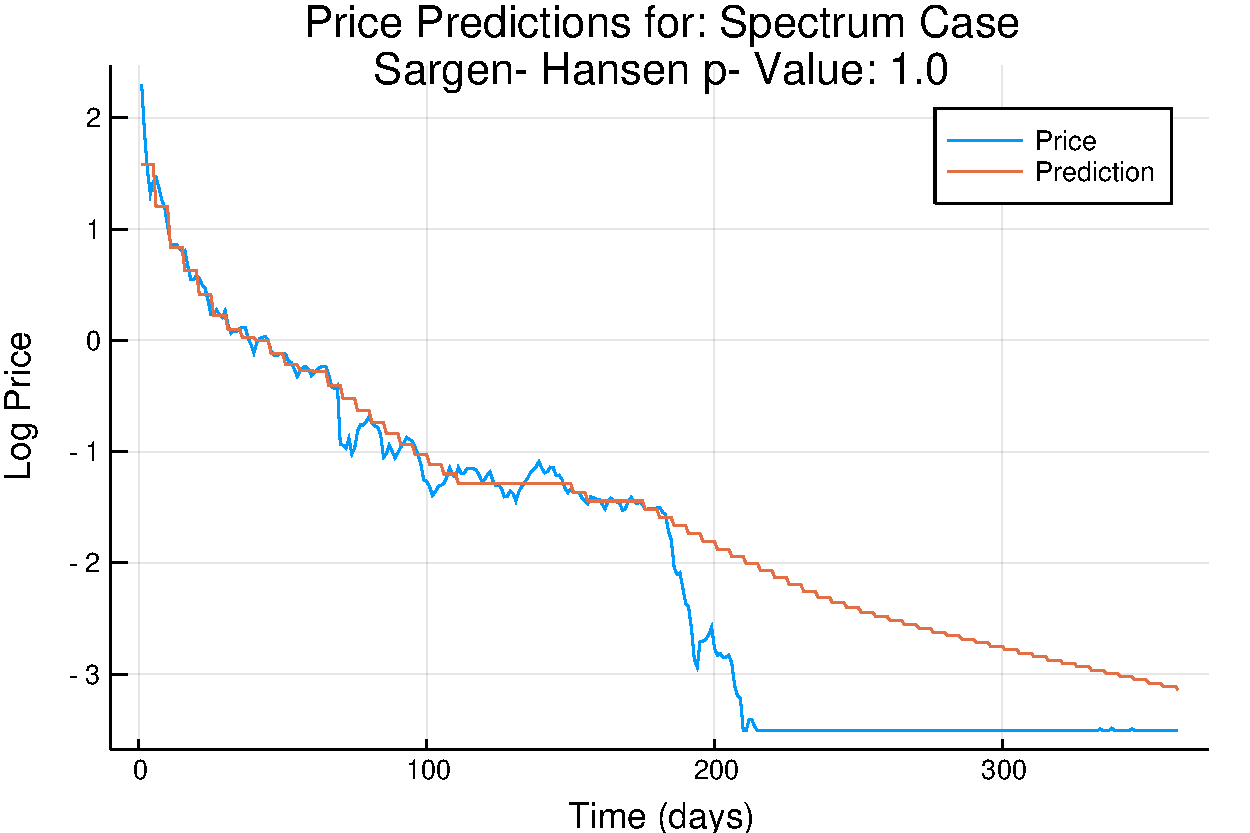
\includegraphics[width=12cm]{../Figures/Cases/Cases2/SpectrumCase.pdf}

\subsection{Monte Carlo Analysis}
\label{sec-4-3}
With these numerical problems in mind, the question of is this
estimation feasible remains. To this end, I simulated the process one
thousand times, and tested the specifications of the simulations under
the model. Since the early values of $\bm{\xi}$ influence the quantity and
price in the later time periods greatly, this allows for noise within
the early stages of the model to propagate down the time intervals.

One thousand simulations were run consisting of one thousand people,
with Log-Normal distributions of $\mu$ = 0, $\sigma$ = 1. In each time period, five
percent of the participants were endowed with the item, and this
continued on for fifty time periods. After each simulation, a J-test
for fitting the model was conducted, as well as a LR test for $\bm{\xi}$ being
constant, and a LR test for the simulation primitives being equal to
what they were. These tests were run at a significance level of $\alpha = 0.05$.

\begin{center}
\begin{tabular}{lrrr}
 & Sargan Hansen & $\bm{\xi}$ constant & Simulation Primitives\\
Reject \% & 3.7 & 44.0 & 100.0\\
\end{tabular}
\end{center}

As one can see, the J-test rejected in an acceptable percent of the
simulations, but the likelihood ratio tests were rejected at a far
higher rate. This simulation is not quite on the order of magnitude of
N as the data is because the linear program required to solve it
scales at a size proportional to the square of the number of
participants. This meant that to simulate at the order of magnitude
for N required would require solving fifty linear programs at a magnitude
of 10$^{\text{14}}$. This means that the simulations are overstating the role of
the random noise compared to the data used, and the LR test for $\bm{\xi}$ may
be slightly more powerful.


\subsection{Testing}
\label{sec-4-4}

Since the model is over-identified, one can test for model-fit using
the J-test for model fit. \cite{hall2005generalized}. Formally, this
entails testing the hypothesis that $M \hat{\bm{m}} ( \hat{\bm{\theta}} )' \widehat{\bm{W}}
\hat{\bm{m}} ( \hat{\bm{\theta}} ) = 0$. Since there are $2T$ moments in the model, and
$T + 3$ primitives in the model, the J-statistic is distributed $\chi^2 (
T - 3 )$.

Of interest is the question of whether or not there has been a
constant drop rate of an item to users in the game over time. This can
be written in the form of: $\bm{\xi} = \bm{1} \xi^c$. That is, $\bm{\xi}$ is constant
over the entire lifetime of the model. This hypothesis can be tested
with a Likelihood-Ratio test. We estimate the model under the null and
compare it to the unconstrained model with the difference in the
J-statistic distributed $\chi^2 ( T - 1 )$ as shown in: \cite{hall2005generalized}.


\begin{center}
\begin{tabular}{llrrrl}
Case & J-test p-Value & LR Test & $\mu$ & $\sigma$ & $N$\\
Clutch & 0.95853 & 0.00140 & 1.47814 & 0.85317 & 1.0 x 10$^{\text{7}}$\\
Glove & 5.02424 x 10$^{\text{-7}}$ & 1.0 & 0.83034 & 1.03382 & 810801.569\\
Gamma & 6.95436 x 10$^{\text{-55}}$ & 0.0 & 1.42149 & 0.42634 & 169083\\
Spectrum 2 & 9.47595 x 10$^{\text{-14}}$ & 1.00000 & 0.50699 & 0.61172 & 278163.43674\\
Operation Hydra & 1.00000 & 1.00000 & 0.79300 & 0.00000 & 9.99999 x 10$^{\text{6}}$\\
Glove & 1.98425 x 10$^{\text{-8}}$ & 0.97342 & 0.76676 & 0.97756 & 899619.98944\\
Spectrum & 1.52588 x 10$^{\text{-22}}$ & 1.00000 & 1.09140 & 0.50655 & 9.99999 x 10$^{\text{6}}$\\
Operation Wildfire & 1.27968 x 10$^{\text{-38}}$ & 1.84931 x 10$^{\text{-8}}$ & 0.59941 & 1.27118 & 658963.25133\\
Revolver & 1.66667 x 10$^{\text{-42}}$ & 0.00044 & 0.94046 & 1.79520 & 896235.25688\\
Gamma 2 & 1.55873 x 10$^{\text{-46}}$ & 1.76041 x 10$^{\text{-54}}$ & 0.49284 & 0.59216 & 464143.69810\\
Huntsman & 3.86569 x 10$^{\text{-5}}$ & 1.62886 x 10$^{\text{-38}}$ & 1.01952 & 0.39789 & 4.30935 x 10$^{\text{6}}$\\
Chroma 2 & 3.02951 x 10$^{\text{-100}}$ & 2.96312 x 10$^{\text{-43}}$ & 1.00659 & 0.51421 & 3.38519 x 10$^{\text{6}}$\\
Winter Offensive & 1.00000 & 1.48174 x 10$^{\text{-120}}$ & 0.94375 & 0.23719 & 2.45622 x 10$^{\text{6}}$\\
Chroma 3 & 4.82901 x 10$^{\text{-65}}$ & 9.96035 x 10$^{\text{-37}}$ & 0.31676 & 0.55150 & 9.48558 x 10$^{\text{6}}$\\
Falchion & 9.50759 x 10$^{\text{-48}}$ & 4.52701 x 10$^{\text{-10}}$ & 0.81208 & 0.84943 & 9.99997 x 10$^{\text{6}}$\\
Shadow & 1.78457 x 10$^{\text{-82}}$ & 4.06310 x 10$^{\text{-16}}$ & 0.58131 & 0.71472 & 9.99996 x 10$^{\text{6}}$\\
Operation Bravo & 1.00000 & 0.00000 & 5.00000 & 0.00000 & 9.99999 x 10$^{\text{6}}$\\
Chroma & 3.12200 x 10$^{\text{-107}}$ & 1.34974 x 10$^{\text{-25}}$ & 1.22655 & 0.61548 & 9.93782 x 10$^{\text{6}}$\\
Operation Vanguard & 1.00000 & 0.00000 & 0.00000 & 0.00000 & 2.57984 x 10$^{\text{8}}$\\
\end{tabular}
\end{center}


One striking result is that in many of the boxes, the LR-test does
reject the possibility that there is an equal endowment process in
many of the boxes. Only in three of the examined boxes, Glove,
Spectrum and Spectrum 2 does the process reject the Null. The other
rejections arise from a poor J-test fit, and no information about the
uniformity of $\bm{\xi}$ can be deduced. While the Glove case contains the
rarest and most expensive items that are obtainable from the cases,
the Spectrum Cases do not. It may be the case that the LR-test
rejected a fit that was actually true, as seen during the Monte-Carlo
simulations, so I believe that there may not be enough information to
deduce a pattern in the boxes that rejected the null
hypothesis. Almost all of the other boxes accept this hypothesis at
virtually all significance levels, determining that random noise is not
causing the differences. Whether the structure imposed has forced
there to be a near equal drop rate is not testable under this model,
but the question remains open.

Almost all the boxes that were rejected at any significance level
reached nearly the same minimizer. For all of them, the mean was
driven as high or low as possible, and the standard deviation as low as
possible. This allowed for the price moment to be as close to matched
as possible, as the path the price took could not be well described by
the structure of the model. At first I believed that fits such as that
were the result of poor initialization of the routine, but I was
unable to find a starting point that did not converge to the same
minimizer. I believe that the price path described by the data simply
cannot be rationalized by the model, as they feature rapidly
increasing prices, and prices rising above their initial price level,
behavior that is completely inexplicable under this model. As a result,
the model fixes the valuations as constant, and attempts to fit the
quantity as best as possible. This is possible because the
distribution of valuations plays no part in the quantity sold.


\subsection{Market Entry}
\label{sec-4-5}
I now consider the possibility of estimation of the market entry process.

\subsubsection{Identification}
\label{sec-4-5-1}
This new model is significantly more complicated and features many new
primitives. For each time period, there are now four primitives. Since
there are only two moments defined per time period, there will need to
be identifying assumptions in order to ensure that there is
identification. The easiest of these assumptions to make is that the
entry distributions are all the same distribution. This assumption is
relatively innocuous and greatly reduces the number of
primitives. However, there remains the 2 primitives of the initial
distribution, as well as the two for the entry distribution, as well as
$T$ for $\bm{\xi}$ and $T$ for $\bm{\lambda}$. One further reduction is to claim that the
distribution of the item has remained constant over time. That is, $\bm{\xi}
= \bm{1} \xi^c$. This reduces our model to one of having $T + 5$
primitives. However, a great deal of structure is imposed in exchange.

The price floor is still present, and is handled in the same way that
it was handled in the model without any entry. For time periods in
which the price floor is binding, the equilibrium condition is not
binding, and the only condition that binds is that the quantity
demanded must be equal to the mass of buyers times the buyer's
distribution function. The same moment is applied.

As long as $T > 5$, then there are enough moments for identification,
so all that must be verified are the conditions for GMM
Estimation. The single crossing property of the competitive equilibria
ensure that $\mathbb{E}[ \bm{m}( Y, \bm{\theta}) ] \neq 0$ for $\bm{\theta} \neq
\bm{\theta_0}$. The only other property required is that the expected value
of the total derivative of $\bm{m}( Y, \bm{\theta} )$ has full rank. This is
assumed under the specification of the model.

\subsubsection{Monte Carlo}
\label{sec-4-5-2}
A serious problem arises with the supply and demand functions when
there is entry allowed within the model. As people re-enter, a small
portion have mass above the previous allowed price. This extends the
mass out near the first price, and in just a few iterations, the supply
and demand curves become extremely flat near the equilibrium price and
quantity. This creates a serious problem for estimation, as tiny
shocks in the distribution can move the price and quantity a large
amount. The numerical problems present in the model without growth are
only exacerbated by the mixing distribution induced in the growth
model. 

A Monte-Carlo simulation was set up with values of $T = 20, \mu_1 = 1, \sigma_1 =
0.5, \lambda_i = 0.05, \xi_i = 0.5, \mu_2 = 2, \sigma_2 = 1$. The buyer and seller
distributions for several of the time periods are shown below:

\begin{figure}
\centering
\begin{minipage}{.5\textwidth}
  \centering
  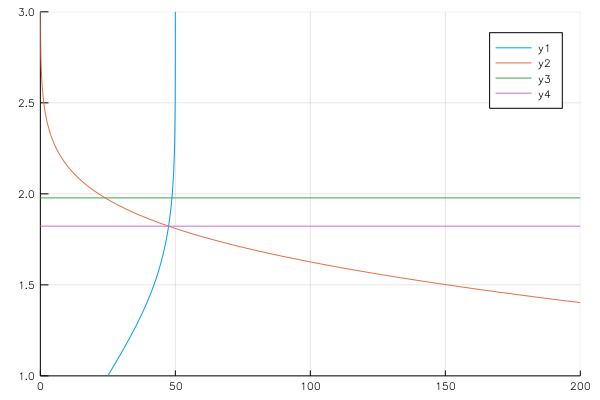
\includegraphics[width=.8\linewidth]{../Figures/gif/000001.png}
  \captionof{figure}{Initial Time Period}
  \label{fig:test1}
\end{minipage}%
\begin{minipage}{.5\textwidth}
  \centering
  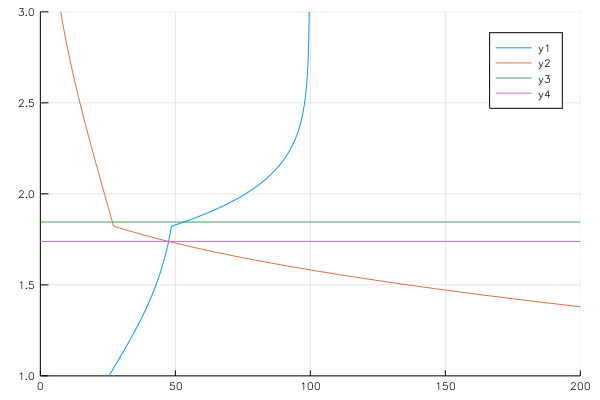
\includegraphics[width=.8\linewidth]{../Figures/gif/000002.png}
  \captionof{figure}{Second Time Period}
  \label{fig:test2}
\end{minipage}
\end{figure}

As one can see, after the first transaction, the distributions become
kinked, but since there are new arrivals with valuations above the
price, the demand distribution does not become truncated as
before. This leads to the recursive definition of the demand and
supply given in the theory. It also complicates the
estimation process greatly, as there are now two variables in the
early time instances that have a great impact upon the model in later
time periods. This means that the estimation process can be very
unstable in the latter time periods, which manifests itself even in a
simulation over 20 time periods.

\begin{figure}
\centering
\begin{minipage}{.5\textwidth}
  \centering
  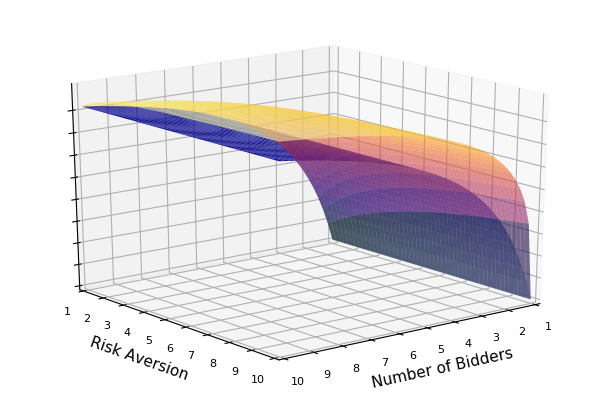
\includegraphics[width=.8\linewidth]{../Figures/gif/000010.png}
  \captionof{figure}{After 10 Time Periods}
  \label{fig:test3}
\end{minipage}%
\begin{minipage}{.5\textwidth}
  \centering
  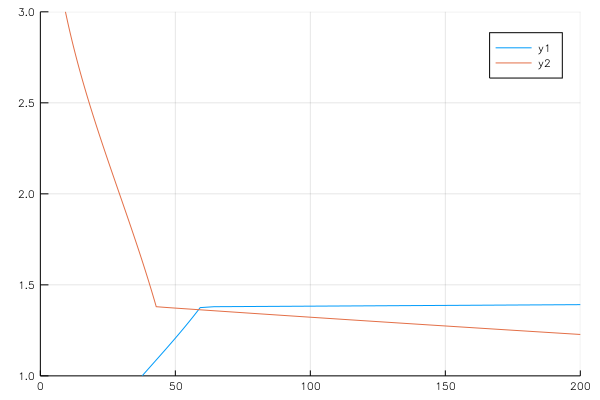
\includegraphics[width=.8\linewidth]{../Figures/gif/000015.png}
  \captionof{figure}{Time Period 15}
  \label{fig:test4}
\end{minipage}
\end{figure}

As one can see, the equilibrium price and quantity are determined by
the intersection between a very flat area of both supply and
demand. This area is extremely sensitive to changes in the price, as
well as noise in the data. For a simulation with $N = 10000$, I was
unable to obtain convergence to any reasonable estimates of the
distribution.

The moments used in estimation were:
\begin{align*}
M_B(T) B_T(p_T^* ) &= M_S(T) S_T(p_T^* )\\
M_B B_T(p_T^* ) &= q_T^*\\
\end{align*}

The same care was taken to avoid problems with the binding price
floor, and numerical problems. In all the simulations, the
numerical problems dominated the process, and even when initialized at
the starting values for the distribution, minimization was always
obtained by setting the standard deviation to infinity, allowing for a
fit in the price moment that way. Because of the numerical issues, as
well as the extreme elasticity in the demand and supply near the
equilibrium price, I do not believe that the estimation of this model
is a possibility. Thus, estimation of other elements of the
process will have to be undertaken in a different direction.


\subsection{Quantile Regression}
\label{sec-4-6}

One initial goal of this paper was to aggregate the cases together,
and introduce covariates into the model. Even with simple
covariates, the optimization procedure would break down with as little
as three or four cases being optimized together through a
scalarization process. Most importantly, due to the structure of this
model, it would not be possible to consider the case where the mean of
the distribution had changed universally among all participants. For
the purposes of estimation, the distribution must be fixed across
time, and each data point must be serially uncorrelated with the other
data points in its moment.

Due to these problems, another approach to the apparent
instability in prices would be useful for policy predictions. In
both models, the price is used to signal the cutoff in the valuations
deciding who obtains an item. Everyone above this quantile receives
the item, either by being endowed, or by trading for it. 

The items in question are random lotteries containing other items of
interest. Instead of believing that each person is identical ex ante
a different draw from an urn of distributions, we could instead
believe that those with different valuations value a different aspect
of the contents of these lotteries. One way to examine how these
affects change over the distribution of prices is to use quantile
regression. The higher quantiles of the price show the behavior of
consumers who have the highest valuations, and bought the item the
soonest. 

Using the fact that quantiles of our model are revealed over time, one
estimate of interest is the conditional quantile. At high quantiles,
when the item is in high demand, we may notice different behavior as
buyers of rare items value different elements.

\subsubsection{Multiple Quantile Regression}
\label{sec-4-6-1}

To this end I employed quantile regression. Even though one can easily apply
quantile regression to a single loot box, and estimate the conditional
quantiles, there is reason to believe that each box does not follow
the same distribution. Thus, it is not immediately possible to simply combine all
the different loot boxes into one data set, using indicators in the X
and estimate the different quantiles.

First consider the optimization problem at the heart of
quantile regression. We seek the quantile function such that: $Q_Y ( \tau
) = F_Y^{-1} (\tau)$. As shown by \cite{10.2307/1913643} it can be found by minimizing the
following function:

\begin{align*}
\hat{\bm{\beta}} = \argmin_{\bm{\beta}} \sum_{n=1}^N \rho_{\tau} ( \bm{Y_i} - \bm{X_i} \bm{\beta} )\\
\end{align*}

This is known to be equivalent to solving the following linear
program:

\begin{align*}
\min \tau \bm{1}' \bm{u} + (1-\tau) \bm{1}' \bm{v} &\\
\bm{X} \bm{\beta} + \bm{u} - \bm{v} &= \bm{Y}\\
\bm{u},\bm{v} &\geq 0
\end{align*}

To estimate the quantile regression estimator for multiple boxes,
consider a world where each box's quantile can be written in the
following form:

$Q_T^i (\tau ) = \bm{X}^i \bm{\beta} + \bm{Z}^i \bm{\delta}^i$. Where $\bm{X}$ and
$\bm{Z}$ are matrices of covariates. Effectively, some covariates are
shared by all boxes, and are contained within the vector $\bm{\beta}$, and some
are unique to each box, and shared by the vector $\bm{\delta}$. We wish to examine
the conditional quantile function of each box, conditioned that each
box must contain the same $\bm{\beta}$. This is a question of multicriterion
optimization. \cite{Boyd:2004:CO:993483}

For the j$^{\text{th}}$ component of the vector to be optimized:
\begin{align*}
\min \left [ \tau \bm{1}' \bm{u_j} + (1-\tau) \bm{1}' \bm{v_j} \right ]&\\
\bm{X_j} \bm{\beta} + \bm{Z_j} \bm{\delta}_j+ \bm{u_j} - \bm{v_j} &= \bm{Y_j} \quad \forall j\\
\bm{u},\bm{v} &\geq 0\\
\end{align*}

By doing this, one chooses the $\bm{\beta}$ that minimizes each of the boxes
residuals. Since there is no reason for us to favor any of the boxes
over the others, we may consider the scalarization with the unit
weight function applied to each of the objectives. Since we are
interested in smallest possible sum of residuals between all boxes,
the unit weight function makes intuitive sense to form our specification.

This effectively is choosing the Pareto Optimal point that has the
smallest magnitude in the u,v space. In English this is the $\bm{\beta}$ value
that allows us the smallest absolute sum of residuals over all the
loot boxes. Since our data is presented as prices and quantities, we
need to weight each of the residuals by this quantity sold, The
scalarization of this problem is readily formed:

\begin{align*}
\min \sum_{j=1}^J \left [ \tau \bm{1}' \bm{u_j} + (1-\tau) \bm{1}' \bm{v_j} \right ]\\
\bm{X_j} \bm{\beta} + \bm{Z_j} \bm{\delta}_j+ \bm{u_j} - \bm{v_j} &= \bm{Y_j} \quad \forall j\\
\bm{u},\bm{v} &\geq 0\\
\end{align*}

This is well-defined optimization problem as it is a Linear Program,
and thus can be solved in $\BigO (N^3)$ run-time. Which is tractable
even for large amounts of data, and can be applied to this model.

\subsubsection{Application}
\label{sec-4-6-2}

The first, and most important covariate for determining the price is
the expected value of the item. The expected value was broken down
into five different components, one for each of the different
qualities. Each case clearly indicates which items it contains as well
as which quality these items have. Each of the qualities was
multiplied by the probability of obtaining that case in order to
ensure that the coefficients were of comparable magnitude. 

Knowing how the price is influenced by the value of the
contents is not particularly useful in designing new cases. Since the
price of the contents is typically controlled by factors related to
tastes that are simply not observed until the case has been
released. What can be controlled easily is the number of items of each
quality contained in each box. For almost all of these cases, there
are between 3-5 items of each quality. So a linearization of the
effect is not creating too large of a misspecification error.

Finally, one important consideration is if the presence of an item will
influence the price. Each item contained is a weapon used within the
game, and certain weapons are used much more often, and thus their
inclusion should influence the price more. Due to the limited
number of cases that have been released however, it is impossible to include
an indicator for every single item in the game, as the corresponding
matrix would not be of full rank. Thus, fifteen of the least popular
weapons have been removed from the regression in order to maintain
linear independence within the model. The chosen weapons are listed in
the table below:

\begin{center}
\begin{tabular}{lllll}
Weapons &  &  &  & \\
AK-47 & AWP & DesertEagle & M4A4 & M4A1-S\\
FAMAS & USP-S & Glock-18 & P250 & P90\\
SG553 & CZ75-Auto & AUG & SSG08 & Five-SeveN\\
MAC-10 & MP7 & MP9 & UMP-45 & \\
\end{tabular}
\end{center}

The model is estimated in R using the package \texttt{quantreg} \cite{quantreg}
contained in the file \texttt{QuantReg.r}. The entire conditional quantile
regression is estimated using multiple quantile regression and using
the Barrodale and Robert's alogrithm \cite{10.2307/3532912}. A technical
problem exists in the R package, preventing large datasets from being
transferred to the internal FORTRAN code. As a result, the lowest
observations were culled from the data set. This eliminated the need
to handle them as censored observations, and allows for the process to
be calculated. We estimate each conditional quantile of the
distribution to be linear in each of the covariates with a single
intercept element. Due to the restrictions in linear independence, no
elements are included in our specification of $\bm{\delta}$, as an
indicator for each lottery would be linearly dependent with the
indicators of items contained.

\subsubsection{Results}
\label{sec-4-6-3}

The coefficients over time for each of the different qualities, as
well as the number of items contained, and the coefficients for the five
most popular items used in game are shown:

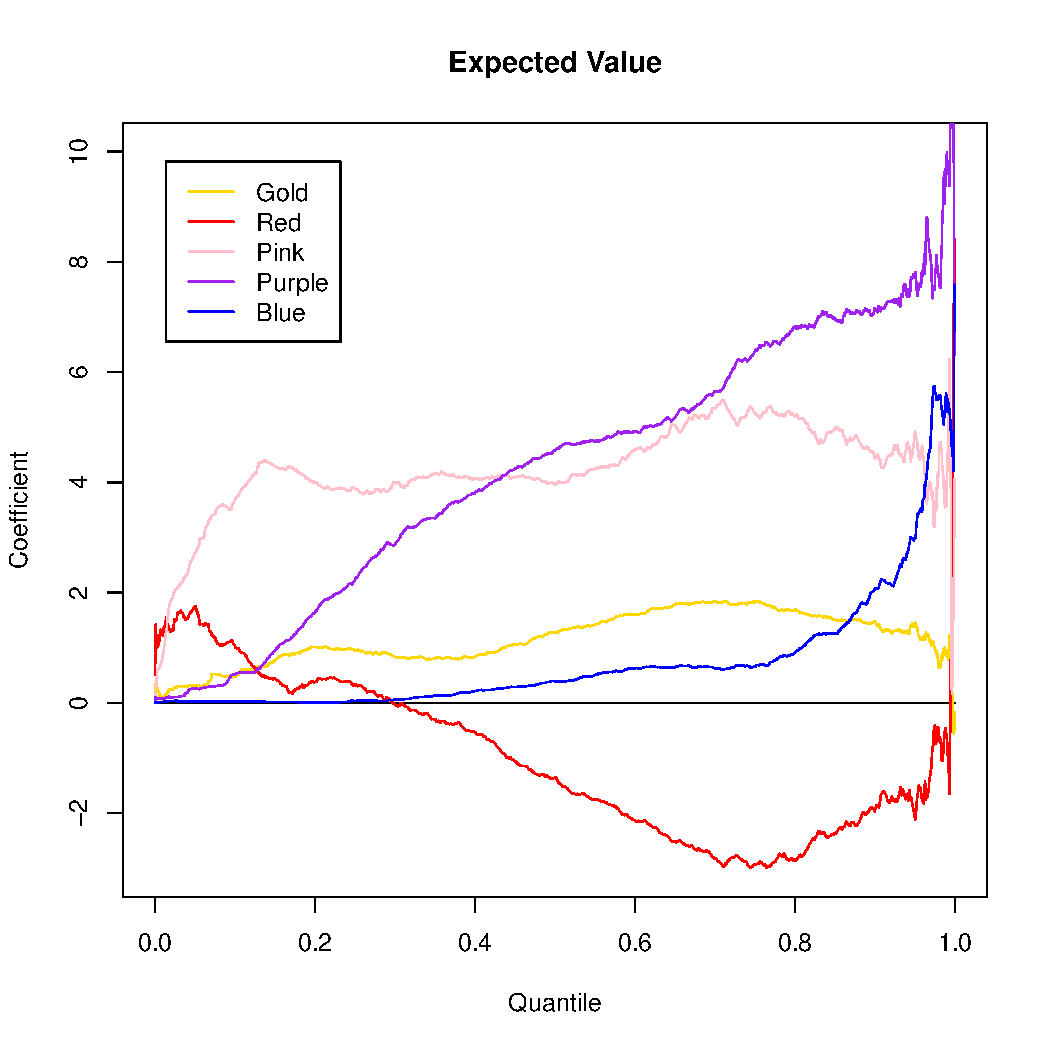
\includegraphics[width=12cm]{../Figures/QuantRegQuality.pdf}

At the lowest quantiles, the results are unexpected, the value of the
rare, but obtainable items (red and pink) weight most heavily on the
value of the item. As the quantile increases, the importance
of the least valuable items rises. This goes against the intuitive
opinion that when the box is least valuable, the value would be
determined by the most commonly obtained items as a kind of
"consolation prize." 

Far more interestingly, is the fact that the coefficient for the red
items dips into negatives for most of the quantiles. This implies that
increases in the expected value of the rare items drive the price
down. One possible interpretation of this result could be that
individuals regard increases in the prices of red items as a decrease
in the supply, lowering the chances of rare items, and driving the
valuation and price down. This requires a strong stance on individuals
beliefs on the market that is not substantiated anywhere. 

Of interest is how by the highest quantiles, when the case is newest,
the value of the least common items dominates the effects of the
others. At this time, when the value of the items contained in the box
is uncertain, individuals are more likely to consider a min-max
approach, and look to the worst case scenarios instead of the rarer
and less certain items.


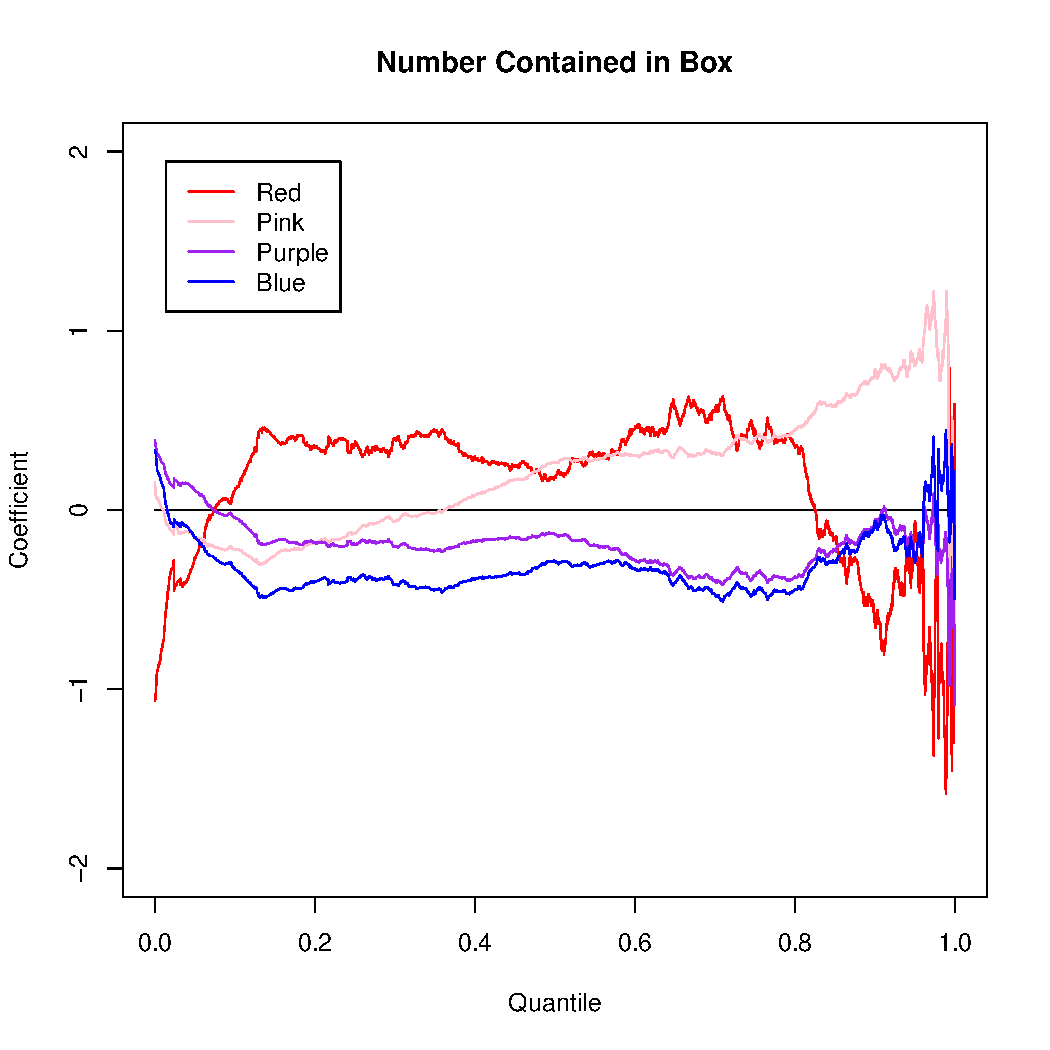
\includegraphics[width=12cm]{../Figures/QuantRegNumInBox.pdf}

For most sales, the number of items of each rarity in each box seems
to have little effect on the price. However, as we reach the top
twenty percent of sales, the value of an additional item increases for
the pink item rises. However, much of these results are not
statistically different from zero, and the behavior at the highest
quantiles is extremely noisy as a result.  Clearly though, additional
items in the rarest categories of the case drive the price up in
almost all quantiles. It must be noted that all the data for the
number contained in the box lies within the range of two to four items
for those rarities. I believe that this pattern would not extend
globally, as individuals seeking a specific item lower their
probability of obtaining it as there are more choices added.


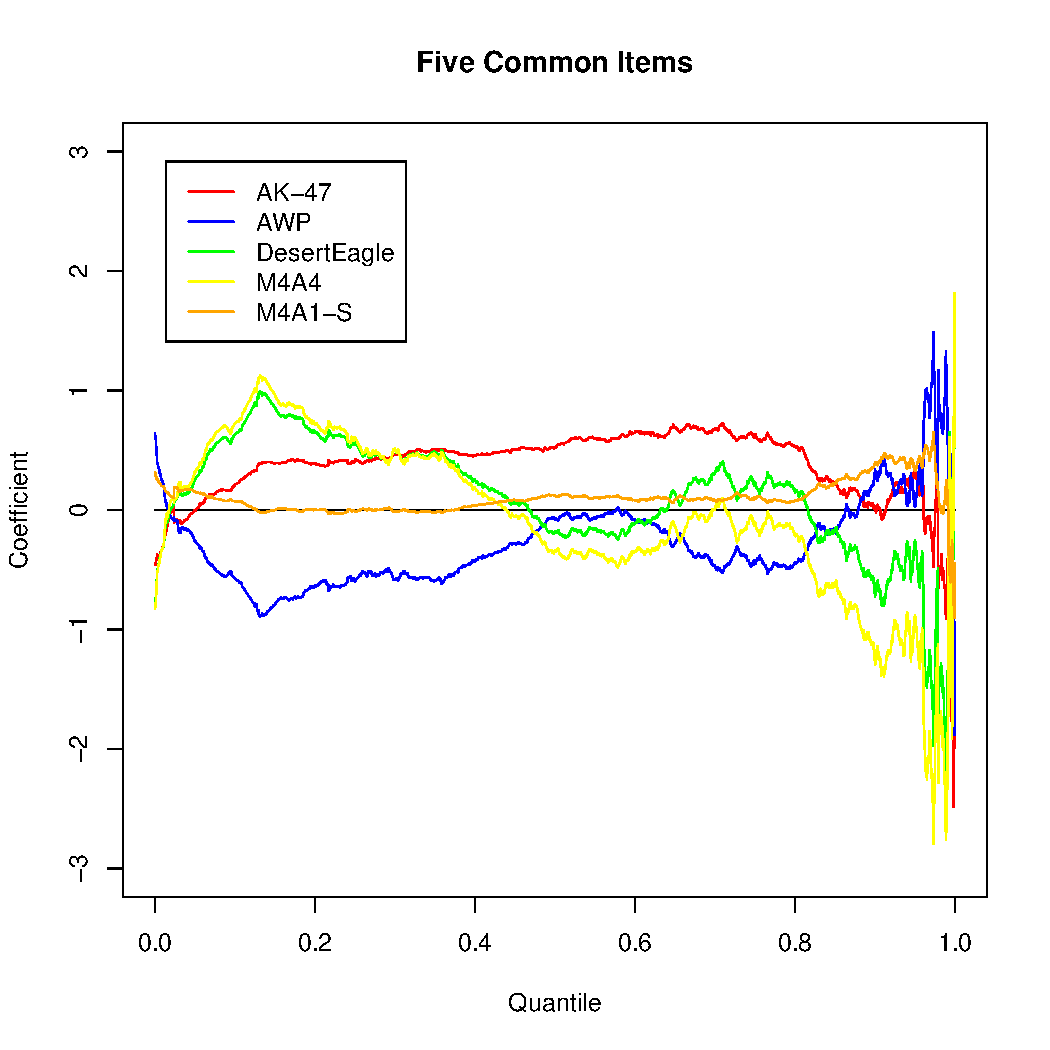
\includegraphics[width=12cm]{../Figures/QuantRegGuns.pdf} 

This plot again suffers from noise and lack of significance at the
highest quantiles for each of the items, and the M4A1-S remains
insignificant at virtually all quantiles. The most striking result
here is that containing the AWP, an item that is very expensive for
all of its varieties and very sought after, drives the price down at
the lower quantiles. While it must be remembered that the inclusion of
the AWP can mean that there is no inclusion of the M4A4 and the AK-47,
the two other weapons that are the most popular. These three items are
never included together in a case, and at most only two of them are
contained within the same case. In the context of the opportunity cost
of including the AWP is losing a more popular weapon, the coefficient
for the AWP can be explained.


\section{Conclusion}
\label{sec-5}

From a policy perspective, the quantile regression suggests that the
most important thing to drive up the revenue earned by the loot boxes
is to drive the value of the common items contained in the box
upwards. This goes against the intuitive thought that by making the
very rare items as desirable as possible, the value of the box will be
driven upward. The inclusion of certain items appears to have as
little of an effect as the number of items contained in the boxes.

For further analysis, a model featuring a linear state space would be
more numerically and computationally sound, and would allow for better
estimation for processes that extend over large time periods. Most
importantly, this model is, in the words of Rothschild, a
"partial-partial equilibrium." \cite{Rothschild} Only the demand side of a
single part of the market is considered. A more complete analysis
would consider the effects of all the markets, beyond simply their
price at the current time period. This model would allow individuals
to form beliefs about prices, and consider a sequential
equilibrium. No consensus exists among Economists for an
equilibrium strategy in a continuous double auction with beliefs about
prices, so this approach presents many problems beyond the scope of
this paper. \cite{DoubleAuc}

An interesting question for further study in this data is whether the
current mechanism (randomization with taxed markets for resale) is
optimal from the perspective of the seller, and what properties are
induced by this mechanism. The uniqueness of this mechanism, as well
as the success it has had in the market seems to suggest that it is
optimal under some conditions that are unique to this world. The
derivation of which would be a very interesting extension.

\section{Data Appendix}
\label{sec-6}
The Data were gathered through the script \texttt{dataPull.py}, and moved
into the sub-directory \texttt{/Data/CSV/}. This data included the price and
quantity history of every single item sold at market in
\emph{Counter-Strike: Global Offensive}.
The data was then placed into a hierarchical file structure by the
script \texttt{MoveFiles.py}. This script sorted each item by its type, skin
and then quality. Certain files were created by hand: text files that
contained the contents of each lottery examined.
\texttt{CreateData.py} then aggregated the prices of each of the contents of
the lottery at each time interval when a lottery was sold with the
probability of it being received as well as its quality and an
indicator for which type of gun it was.
This data was then used by \texttt{newDataRead.jl} Where the expected values
and other covariates for quantile regression were calculated. The
quantile regression was undertaken in the file \texttt{quantRegR.r}.
The remaining files were altered by \texttt{dateAdjuster.py} to make the date
format amenable to julia's \texttt{DataFrames} Package. These files were then
used by \texttt{dataTest2.jl} to estimate the structural model.

A sample of one file pulled using \texttt{dataPull.py} is as follows:

\begin{center}
\begin{tabular}{rrr}
Date & Price & Quantity\\
15-10-16 & 0.054 & 42502\\
16-10-16 & 0.045 & 38618\\
17-10-16 & 0.051 & 31563\\
18-10-16 & 0.053 & 32452\\
19-10-16 & 0.052 & 36564\\
20-10-16 & 0.049 & 35290\\
21-10-16 & 0.048 & 43502\\
22-10-16 & 0.047 & 38081\\
23-10-16 & 0.04 & 39843\\
24-10-16 & 0.036 & 32493\\
25-10-16 & 0.042 & 30841\\
\end{tabular}
\end{center}

A sample of one row from the files generated by \texttt{CreateData.py}, the
first row of the Revolver Case:


\begin{center}
\begin{tabular}{rrrr}
Case Price: & 8.262 & Case Quantity: & 132808\\
Price & Probability & Rarity & WeaponID\\
142.576 & 0.00043333 & 1 & -1\\
57.309 & 0.00043333 & 1 & -1\\
64.017 & 0.00043333 & 1 & -1\\
161.424 & 0.00043333 & 1 & 14\\
232.763 & 0.00043333 & 1 & -1\\
230.35 & 0.00043333 & 1 & -1\\
123.516 & 0.00049778 & 2 & 25\\
77.369 & 0.00056889 & 2 & 25\\
49.229 & 0.00163556 & 2 & 25\\
48.541 & 0.00049778 & 2 & 25\\
105.682 & 0.000224 & 2 & 13\\
46.822 & 0.000256 & 2 & 13\\
21.616 & 0.000736 & 2 & 13\\
20.323 & 0.000224 & 2 & 13\\
14.833 & 0.00176 & 2 & 13\\
53.181 & 0.00074667 & 3 & 0\\
38.945 & 0.00085333 & 3 & 0\\
26.673 & 0.00245333 & 3 & 0\\
23.986 & 0.00074667 & 3 & 0\\
15.222 & 0.00586667 & 3 & 0\\
16.153 & 0.00201802 & 3 & 23\\
5.893 & 0.00663063 & 3 & 23\\
5.231 & 0.00201802 & 3 & 23\\
35.978 & 0.00091756 & 3 & 8\\
5.53 & 0.00263799 & 3 & 8\\
4.775 & 0.00080287 & 3 & 8\\
4.787 & 0.00630824 & 3 & 8\\
6.281 & 0.00186433 & 4 & 24\\
3.21 & 0.00213067 & 4 & 24\\
1.8 & 0.00612567 & 4 & 24\\
1.469 & 0.00186433 & 4 & 24\\
1.345 & 0.01464833 & 4 & 24\\
2.624 & 0.00304381 & 4 & 19\\
1.382 & 0.00266333 & 4 & 19\\
1.371 & 0.02092619 & 4 & 19\\
8.324 & 0.00186433 & 4 & 7\\
3.951 & 0.00213067 & 4 & 7\\
2.211 & 0.00612567 & 4 & 7\\
1.651 & 0.00186433 & 4 & 7\\
1.454 & 0.01464833 & 4 & 7\\
7.802 & 0.00490614 & 4 & 28\\
3.002 & 0.00560702 & 4 & 28\\
1.786 & 0.01612018 & 4 & 28\\
10.971 & 0.00186433 & 4 & 30\\
5.421 & 0.00213067 & 4 & 30\\
\end{tabular}
\end{center}

\begin{center}
\begin{tabular}{rrrr}
Price & Probability & Rarity & WeaponID\\
3.143 & 0.00612567 & 4 & 30\\
2.614 & 0.00186433 & 4 & 30\\
1.888 & 0.01464833 & 4 & 30\\
3.666 & 0.00242121 & 4 & 33\\
2.552 & 0.0027671 & 4 & 33\\
1.519 & 0.00242121 & 4 & 33\\
1.455 & 0.01902381 & 4 & 33\\
33.066 & 0.009324 & 5 & 25\\
10.289 & 0.010656 & 5 & 25\\
4.782 & 0.030636 & 5 & 25\\
4.42 & 0.009324 & 5 & 25\\
2.821 & 0.07326 & 5 & 25\\
1.506 & 0.009324 & 5 & 1\\
0.657 & 0.010656 & 5 & 1\\
0.34 & 0.030636 & 5 & 1\\
0.526 & 0.009324 & 5 & 1\\
0.285 & 0.07326 & 5 & 1\\
1.006 & 0.02072 & 5 & 4\\
0.675 & 0.02368 & 5 & 4\\
0.481 & 0.06808 & 5 & 4\\
0.6 & 0.02072 & 5 & 4\\
0.915 & 0.02453684 & 5 & 21\\
0.66 & 0.02804211 & 5 & 21\\
0.563 & 0.08062105 & 5 & 21\\
0.882 & 0.01351304 & 5 & 26\\
0.282 & 0.01351304 & 5 & 26\\
0.276 & 0.10617391 & 5 & 26\\
0.657 & 0.01210909 & 5 & 27\\
0.444 & 0.01383896 & 5 & 27\\
0.297 & 0.01210909 & 5 & 27\\
0.286 & 0.09514286 & 5 & 27\\
\end{tabular}
\end{center}



\newpage 

\section{Bibliography}
\label{sec-7}

\nocite{Efficiency}
\nocite{LimeBoy}
\nocite{PriceDataOnly}
\nocite{LitReview}
\nocite{Liquidpedia}
\nocite{SteamMarket}
\nocite{NonAtomic}
\nocite{StructuralEconometrics}

\bibliography{biblio}
% Emacs 25.3.1 (Org mode 8.2.10)
\end{document}